\documentclass[a4paper,11pt]{article}

\usepackage[utf8]{inputenc}
\usepackage[T1]{fontenc}
\usepackage{lmodern}
\usepackage[a4paper,margin=2.6cm]{geometry}
\usepackage{graphicx}
\usepackage{float}
\usepackage{hyperref}
\usepackage{booktabs}
\usepackage{amsmath}
\usepackage{siunitx}
\usepackage{xcolor}
\usepackage{listings}
\usepackage{enumitem}
\usepackage{caption}
\usepackage{titlesec}
\usepackage{fancyhdr}
\usepackage{tcolorbox}
\usepackage{array}

% ----- Colors -----
\definecolor{bluepoli}{cmyk}{0.4,0.1,0,0.4}
\definecolor{lightbluepoli}{RGB}{235,242,250}
\definecolor{todobg}{RGB}{248,248,248}
\definecolor{todoframe}{RGB}{180,180,180}

% ----- Hyperref -----
\hypersetup{
    colorlinks=true,
    linkcolor=bluepoli,
    urlcolor=bluepoli,
    citecolor=bluepoli
}

% ----- Section style -----
\titleformat{\section}
{\color{bluepoli}\normalfont\Large\bfseries}
{\thesection}{0.8em}{}

\titleformat{\subsection}
{\color{bluepoli}\normalfont\large\bfseries}
{\thesubsection}{0.8em}{}

\titleformat{\subsubsection}
{\color{bluepoli}\normalfont\normalsize\bfseries}
{\thesubsubsection}{0.8em}{}

% ----- Caption style -----
\captionsetup{
    labelfont={color=bluepoli,bf},
    textfont=it
}

% ----- Header / footer -----
\pagestyle{fancy}
\fancyhf{}
\fancyhead[L]{\textcolor{bluepoli}{IoT Challenge 1}}
\fancyhead[R]{\textcolor{bluepoli}{ESP32 Motion Sensor Node}}
\fancyfoot[C]{\thepage}
\setlength{\headheight}{14pt}

% ----- Code style -----
\lstset{
    basicstyle=\ttfamily\small,
    breaklines=true,
    frame=single,
    columns=fullflexible,
    backgroundcolor=\color{lightbluepoli},
    rulecolor=\color{bluepoli},
    keywordstyle=\color{bluepoli}\bfseries,
    commentstyle=\itshape\color{gray},
    showstringspaces=false
}

% ----- TODO box -----
\newtcolorbox{todobox}{
    colback=todobg,
    colframe=todoframe,
    boxrule=0.5pt,
    arc=2mm,
    left=2mm,
    right=2mm,
    top=1mm,
    bottom=1mm
}

\newcommand{\TODO}[1]{
\begin{todobox}
\textbf{TODO:} #1
\end{todobox}
}

% ----- Title -----
\title{
    \vspace{-1cm}
    {\Huge\textcolor{bluepoli}{IoT Challenge 1}}\\[0.4cm]
    {\Large ESP32 Motion Sensor Node}
}
\author{
    Marco Abbadessa - 10854816 \\
    Alice Berta - 10889590
}
\date{Academic Year 2025--2026}

\begin{document}

\maketitle
\thispagestyle{empty}

\vspace{0.5cm}
\tableofcontents
\newpage

% ============================================================
\section{Introduction}
% ============================================================

The aim of this work is to design and emulate an IoT motion sensor node for a
smart-home scenario. The node is based on an ESP32 board and is required to detect
human motion through a PIR sensor, while also estimating the ambient light level
through a photoresistor. The collected information is then transmitted to a sink node,
which can use it to support decisions such as turning on or off the lights in the room.\\

According to the challenge specifications, communication must be implemented through
the ESP-NOW protocol. Moreover, the sink node can be considered always reachable. To
reduce energy consumption, the sensor node does not operate continuously. Instead, it
follows a duty-cycled strategy: after sensing and transmitting, the ESP32 enters Deep
Sleep for a fixed interval, then wakes up, and repeats the same execution flow.\\

The output message generated by the node must follow one of the two required formats:
\begin{itemize}
    \item \texttt{MOTION\_DETECTED-LUMINOSITY:ZZZ}
    \item \texttt{MOTION\_NOT\_DETECTED-LUMINOSITY:ZZZ}
\end{itemize}

In the implemented solution, the board periodically reads the state of a PIR sensor
and the light value acquired through an LDR-based circuit, combines them into the
required string, transmits the result using ESP-NOW, and finally enters Deep Sleep.
This design reflects the typical behavior of battery-powered IoT sensing devices,
where the active phase must be kept as short as possible and most of the lifetime is
spent in a low-power state.

% ============================================================
\section{Hardware Design}
% ============================================================

The hardware architecture developed in Wokwi is intentionally simple and includes
only the components required by the challenge: an ESP32 development board, a PIR
motion sensor, and a photoresistor used to estimate ambient brightness.\\

The PIR sensor is connected to GPIO13 and is used as a digital input device. Its
output directly indicates whether motion is detected in the monitored environment.
Since the PIR sensor provides a binary signal, it is particularly suitable for
distinguishing between the two states required by the challenge, namely motion
detected and motion not detected.\\

The ambient light level is measured through a photoresistor connected to the analog
input GPIO34. In practice, the LDR is used within a voltage-divider configuration
with a 10\,k$\Omega$ resistor, so that the ESP32 can observe a voltage that varies
with light intensity. This analog value is then converted through the board ADC and
used as the luminosity field of the transmitted message.\\

The complete node is therefore composed of:
\begin{itemize}
    \item one ESP32 board;
    \item one PIR sensor connected to GPIO13;
    \item one photoresistor connected to GPIO34.
\end{itemize}

This hardware configuration is sufficient to satisfy the sensing requirements of the
challenge while keeping the system compact and easy to analyze.

\begin{figure}[H]
    \centering
    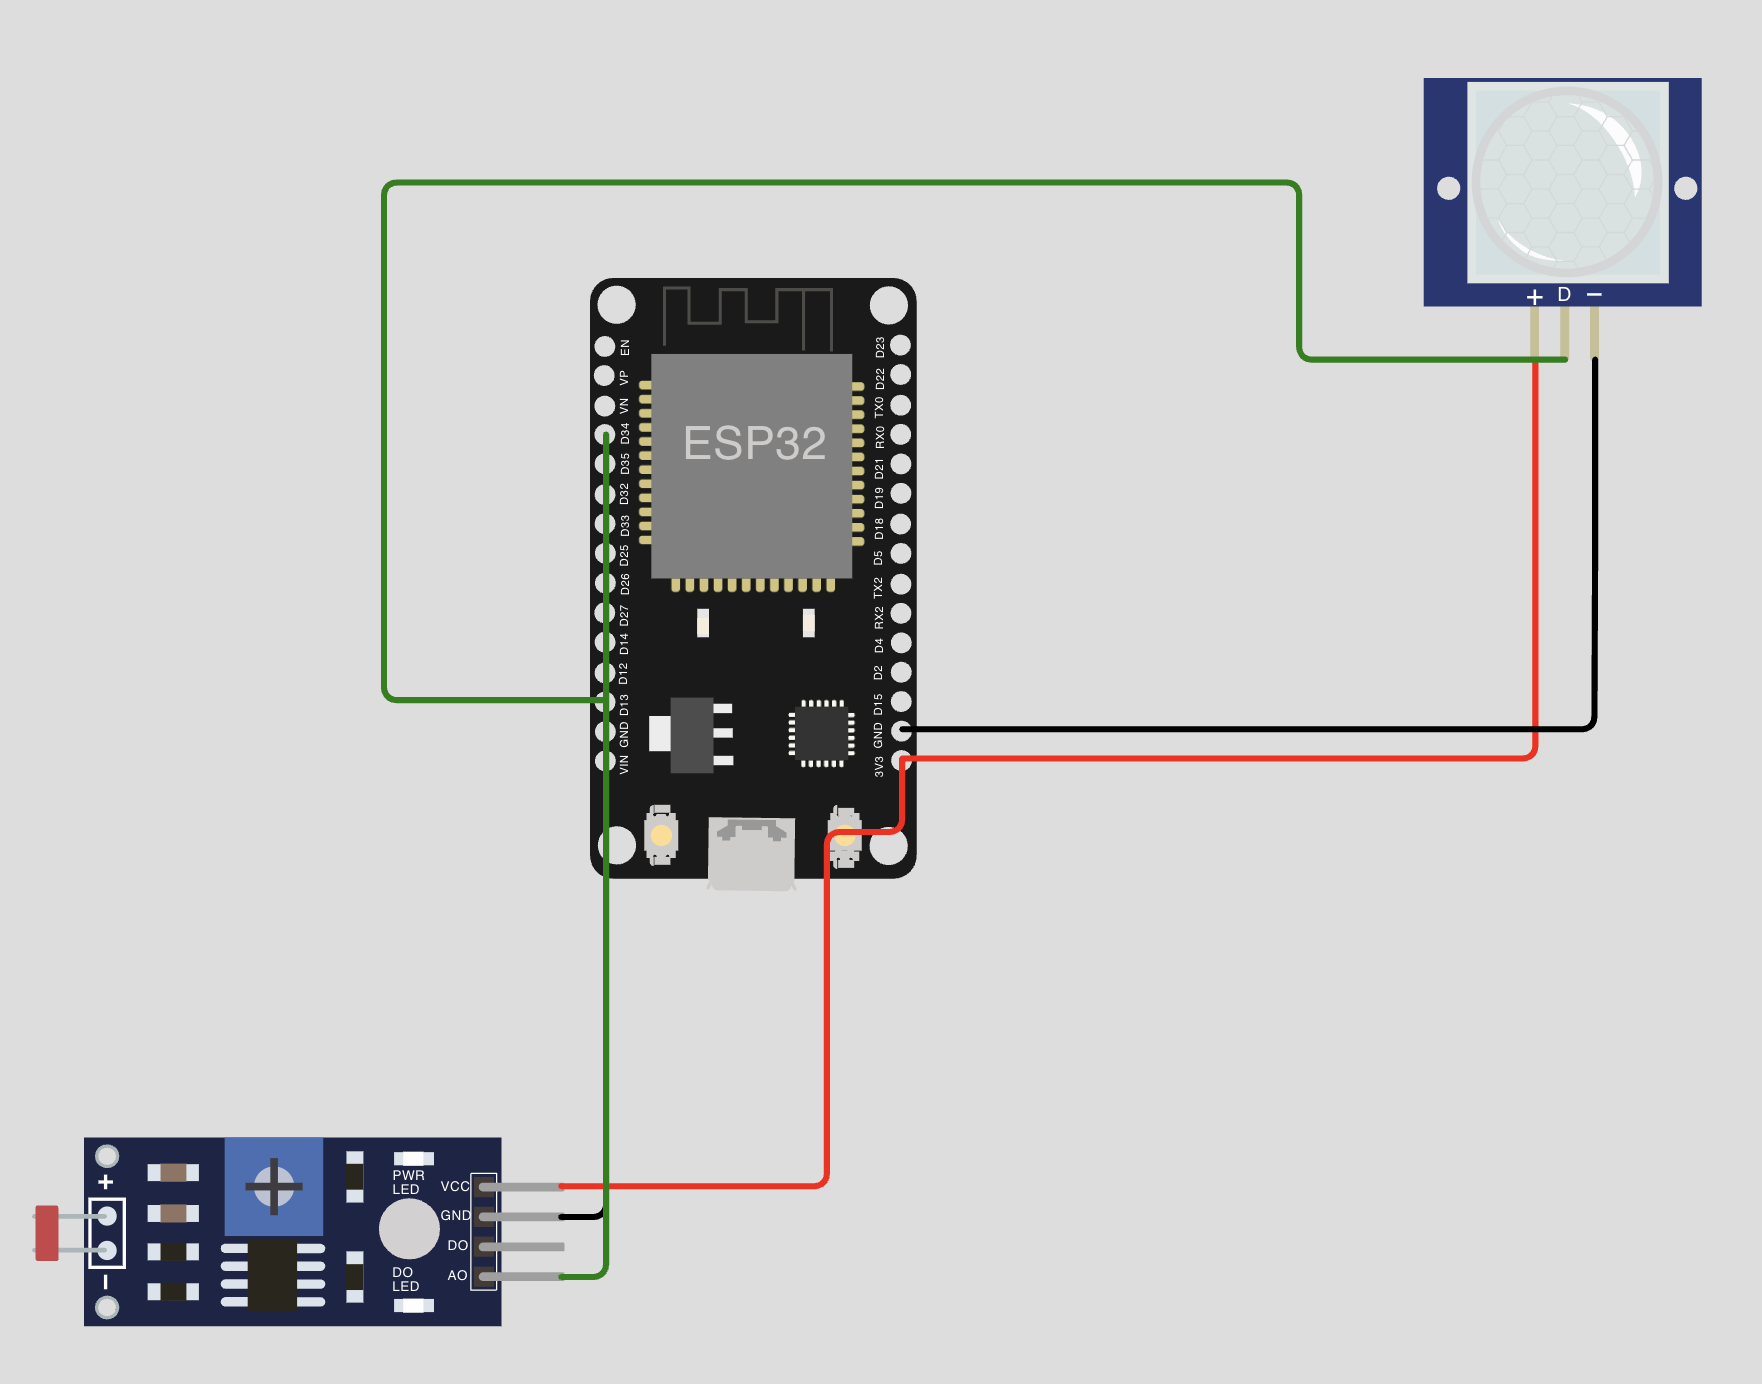
\includegraphics[width=0.68\textwidth]{image/circuit.png}
    \caption{Wokwi schematic of the ESP32 motion sensor node.}
    \label{fig:circuit}
\end{figure}

% ============================================================
\section{Software Design}
% ============================================================

The software was designed according to the duty-cycled operating model required by
the challenge. The core logic is not divided between \texttt{setup()} and
\texttt{loop()}. Instead, the entire behavior of the node is implemented inside
\texttt{setup()}, while \texttt{loop()} is intentionally left empty.\\

This choice is not accidental, but directly follows from the behavior of the ESP32
in Deep Sleep mode. When the board wakes up from Deep Sleep, it does not resume
execution from the point where it was suspended. Instead, it performs a full reset
and starts again from the beginning of \texttt{setup()}. For this reason, the
\texttt{loop()} function is never actually used as the core execution point of the
application.\\

At the beginning of each cycle, the board initializes the serial interface with\\
\texttt{Serial.begin(115200)} and waits one second before printing diagnostic
messages. This delay ensures that the serial monitor is ready before the debugging
output is emitted. The code then increments and prints a boot counter and reports
the wake-up reason.\\

The boot counter is declared as:

\begin{lstlisting}
RTC_DATA_ATTR int bootCount = 0;
\end{lstlisting}

The \texttt{RTC\_DATA\_ATTR} attribute stores the variable in RTC memory, which is
the only memory area that survives Deep Sleep on real ESP32 hardware. Therefore, on a
physical board the boot counter would increase across wake-up cycles. In Wokwi,
however, RTC memory is not preserved correctly across Deep Sleep cycles, so the
variable may appear to reset and remain equal to 1 at each restart.\\

At each activation cycle, the program executes the following operations:
\begin{enumerate}
    \item low-level initialization and diagnostic output;
    \item acquisition of motion and light data from the sensors;
    \item generation of the output message in the required format;
    \item activation of WiFi in station mode and initialization of ESP-NOW;
    \item transmission of the message to the sink node;
    \item transition to Deep Sleep for the programmed time interval.
\end{enumerate}

\subsection{Low-Level Initialization}

Some low-level ESP32-specific headers are included in the project, namely
\texttt{soc/soc.h} and \texttt{soc/rtc\_cntl\_reg.h}. These are needed because the
code directly accesses the brownout detector control register through:\\

\begin{lstlisting}
WRITE_PERI_REG(RTC_CNTL_BROWN_OUT_REG, 0);
\end{lstlisting}

The brownout detector is a hardware safety mechanism that resets the ESP32 when the
supply voltage falls below a critical threshold. In this project it is disabled
because enabling WiFi and ESP-NOW may produce a short current spike, especially in
battery-powered operation, which can momentarily lower the voltage and trigger an
undesired reset even when the system is otherwise functioning correctly. In a real
commercial product this choice would require more caution, but in a simulated
environment and in an experimental prototype it is a common practical workaround to
avoid spurious resets during transmission.

\subsection{Sensor Acquisition}

The PIR sensor is read through \texttt{digitalRead()}, producing a boolean value that
indicates whether motion is present. This allows the software to select the correct
textual prefix for the outgoing message.\\

The photoresistor is read through \texttt{analogRead()}. Before the acquisition, the
ADC resolution is configured to 12 bits by calling \texttt{analogReadResolution(12)}.
Consequently, the measured luminosity value ranges from 0 to 4095 and can be
interpreted as a numerical estimate of the ambient brightness level.

\subsection{Message Formatting}

Once both sensor values have been acquired, the software builds the output string
according to the format required by the challenge.\\

\begin{lstlisting}[language=C++]
String msg = motion
  ? "MOTION_DETECTED-LUMINOSITY:" + String(lux)
  : "MOTION_NOT_DETECTED-LUMINOSITY:" + String(lux);
\end{lstlisting}

This solution guarantees that each transmitted packet strictly follows the required
syntax.

\subsection{Communication Initialization}

After the sensing phase, the ESP32 enables WiFi in station mode by calling
\texttt{WiFi.mode(WIFI\_STA)}, which is required in order to use ESP-NOW. The code
then initializes the ESP-NOW subsystem, registers the transmission callback, and adds
a peer associated with the broadcast address.\\

The broadcast MAC address is:

\begin{lstlisting}
uint8_t broadcastAddress[] = {0xFF, 0xFF, 0xFF, 0xFF, 0xFF, 0xFF};
\end{lstlisting}

Using \texttt{FF:FF:FF:FF:FF:FF} makes it possible to send the packet to all ESP-NOW
devices within range without knowing in advance the specific MAC address of the sink
node. The \texttt{peerInfo} structure is the internal ESP-NOW data structure used to
register the destination peer before transmission.\\

An important implementation detail is that WiFi and ESP-NOW are initialized only
after sensor acquisition has already been completed. This is a deliberate design
choice: since radio activation is the most expensive phase in terms of energy,
postponing it until it is strictly necessary helps reduce the duration of the costly
active phase.

\subsection{Deep Sleep}

Once the packet has been sent, the node prints a final diagnostic message, configures
the wake-up timer, flushes the serial buffer, and enters Deep Sleep:\\

\begin{lstlisting}[language=C++]
esp_sleep_enable_timer_wakeup(TIME_TO_SLEEP * uS_TO_S_FACTOR);
Serial.flush(); // Flush serial buffer before sleeping
esp_deep_sleep_start(); // Enter deep sleep
\end{lstlisting}

The wake-up timer must be expressed in microseconds, hence the multiplication by the
conversion factor. In the current implementation, the sleep interval is set to
4.5 seconds, coherently with the challenge formula used for the value~$X$.\\

After \texttt{esp\_deep\_sleep\_start()} is executed, the ESP32 powers down almost
all of its internal components and only the RTC domain remains active. When the timer
expires, the chip restarts from the beginning of \texttt{setup()}, which is why the
whole execution flow is designed as a self-contained cycle.

\subsection{Wake-Up Diagnostics}

A utility function is used to inspect the wake-up reason through
\texttt{esp\_sleep\_get\_wakeup\_cause()} and print it on the serial interface. On
real hardware, after the first boot the wake-up cause should be reported as
timer-based wake-up. In Wokwi, however, this information is not always reproduced
faithfully, and the serial output may still show a generic message such as power-on
or reset.\\

Nevertheless, the simulator output also reports the reset code \texttt{rst:0x8}
(\texttt{TG1WDT\_SYS\_RESET}), which confirms that the reset is actually produced by
the Deep Sleep timer.

% ============================================================
\section{Timing Measurements}
% ============================================================

In order to support the energy analysis developed later in the report, the duration
of the main execution phases was measured in Wokwi using the \texttt{micros()}
function, as explicitly suggested by the challenge instructions.\\

The measurements were repeated over multiple cycles. The first cycle is affected by
cold-boot effects (a \texttt{POWERON\_RESET} that requires a more complete WiFi
initialization, taking approximately 216\,ms instead of the nominal 196\,ms). The
second cycle shows an additional anomaly caused by a MAC calibration issue: the
simulator does not preserve flash memory correctly between Deep Sleep cycles, so the
ESP32 finds inconsistent data and must recalibrate, taking approximately 228\,ms.
From the third cycle onward, the behavior becomes stable and the timing values can be
considered representative of normal operation. All figures reported in this section
are averaged over the stable cycles only.\\

The average measured durations are summarized in Table~\ref{tab:timings}.

\begin{table}[H]
\centering
\begin{tabular}{>{\raggedright\arraybackslash}p{7cm}r}
\toprule
\textbf{Phase} & \textbf{Average duration} \\
\midrule
Boot delay (\texttt{delay(1000)})   & 1000\,ms \\
Sensor reading                       &  0.43\,ms \\
WiFi + ESP-NOW initialization        & 196.0\,ms \\
Transmission (incl.\ \texttt{delay(100)}) & 99.3\,ms \\
Deep Sleep                           & 4500\,ms \\
\midrule
Total active time                    & $\approx$1296\,ms \\
Total cycle duration                 & $\approx$5796\,ms \\
Active fraction                      & $\approx$22\% \\
\bottomrule
\end{tabular}
\caption{Average timing values measured in Wokwi (stable cycles only, cycles 1--2
excluded). The boot delay is not measured by \texttt{micros()}.}
\label{tab:timings}
\end{table}

The sensor-reading phase is highly stable, with values consistently around
429--430\,$\mu$s across repeated cycles, confirming that sensing is both fast and
reliable. The WiFi and ESP-NOW initialization stage is significantly longer, since
enabling the radio subsystem and configuring communication introduces a substantial
overhead. The transmission phase requires careful interpretation: the measured TX time
does not correspond only to the actual packet transmission, because the timing window
includes both the call to \texttt{esp\_now\_send()} and a fixed \texttt{delay(100)}
introduced to ensure that the send callback completes before the node enters Deep
Sleep. Therefore, the reported value of approximately 99.3\,ms should be understood
as a synchronization interval rather than as the pure physical transmission latency.\\

The boot delay of 1000\,ms, executed immediately after \texttt{Serial.begin()}, is
not captured by the \texttt{micros()} measurements since it precedes all timed
sections. It is nonetheless real active time and is therefore included in the total
figures above. Summing all active phases, the ESP32 is awake for approximately
1296\,ms per cycle and spends the remaining 4500\,ms in Deep Sleep, yielding an
active fraction of approximately 22\%.

% ============================================================
\section{Energy Consumption Estimation}
% ============================================================

The average power drawn during each operating phase was extracted from the 
pre-recorded power-consumption CSV files provided for the challenge. Three CSV files were analyzed, covering the sensor-reading phase (\texttt{sensor\_read.csv}), the WiFi initialization
and transmission phase (\texttt{sender.csv}), and the Deep Sleep phase
(\texttt{deep\_sleep.csv}). \\

To accurately isolate the consumption of distinct operational 
states from the raw data, a custom Python script utilizing the \texttt{pandas} library 
was developed. Rather than computing a simple global mean, the script applied power thresholds to filter the data traces, effectively separating overlapping states
(e.g., distinguishing the high-power WiFi initialization phase from the subsequent 
transmission peak and baseline idle currents). The resulting mean power values 
associated with each phase of the duty cycle are reported in Table~\ref{tab:energy}.

\begin{table}[H]
\centering
\begin{tabular}{>{\raggedright\arraybackslash}p{6.5cm}rrl}
\toprule
\textbf{Phase} & \textbf{Avg.\ power} & \textbf{Duration} & \textbf{Energy} \\
\midrule
Boot delay                    & 252.22\,mW &  1000\,ms & 0.2522\,J \\
Sensor acquisition            & 238.02\,mW &  0.43\,ms & 0.0001\,J \\
WiFi + ESP-NOW initialization & 632.04\,mW &  196\,ms  & 0.1238\,J \\
Transmission (19.5\,dBm)      & 687.93\,mW &  99.3\,ms & 0.0683\,J \\
Deep Sleep                    &  45.78\,mW & 4500\,ms  & 0.2060\,J \\
\midrule
Total per cycle               &   ---   & 5796\,ms  & 0.6504\,J \\
\bottomrule
\end{tabular}
\caption{Energy estimation for one duty cycle. Power values are derived from the
simulation CSV traces. The sensor acquisition energy is below 0.001\,J and is
shown as 0.000\,J after rounding.}
\label{tab:energy}
\end{table}

The dominant contribution to total energy per cycle is the boot delay, which alone
accounts for 0.2522\,J out of 0.6504\,J (nearly 39\% of the total) despite being
simply an idle wait. The WiFi and ESP-NOW initialization phase is the second largest
consumer at 0.124\,J, driven by the high power draw of the radio subsystem during
startup. The Deep Sleep phase contributes 0.206\,J because, although the instantaneous
power is very low (46\,mW), the sleep interval is long enough that its total energy is
non-negligible. Sensor acquisition is almost negligible, lasting less than half a millisecond.

\begin{figure}[H]
    \centering
    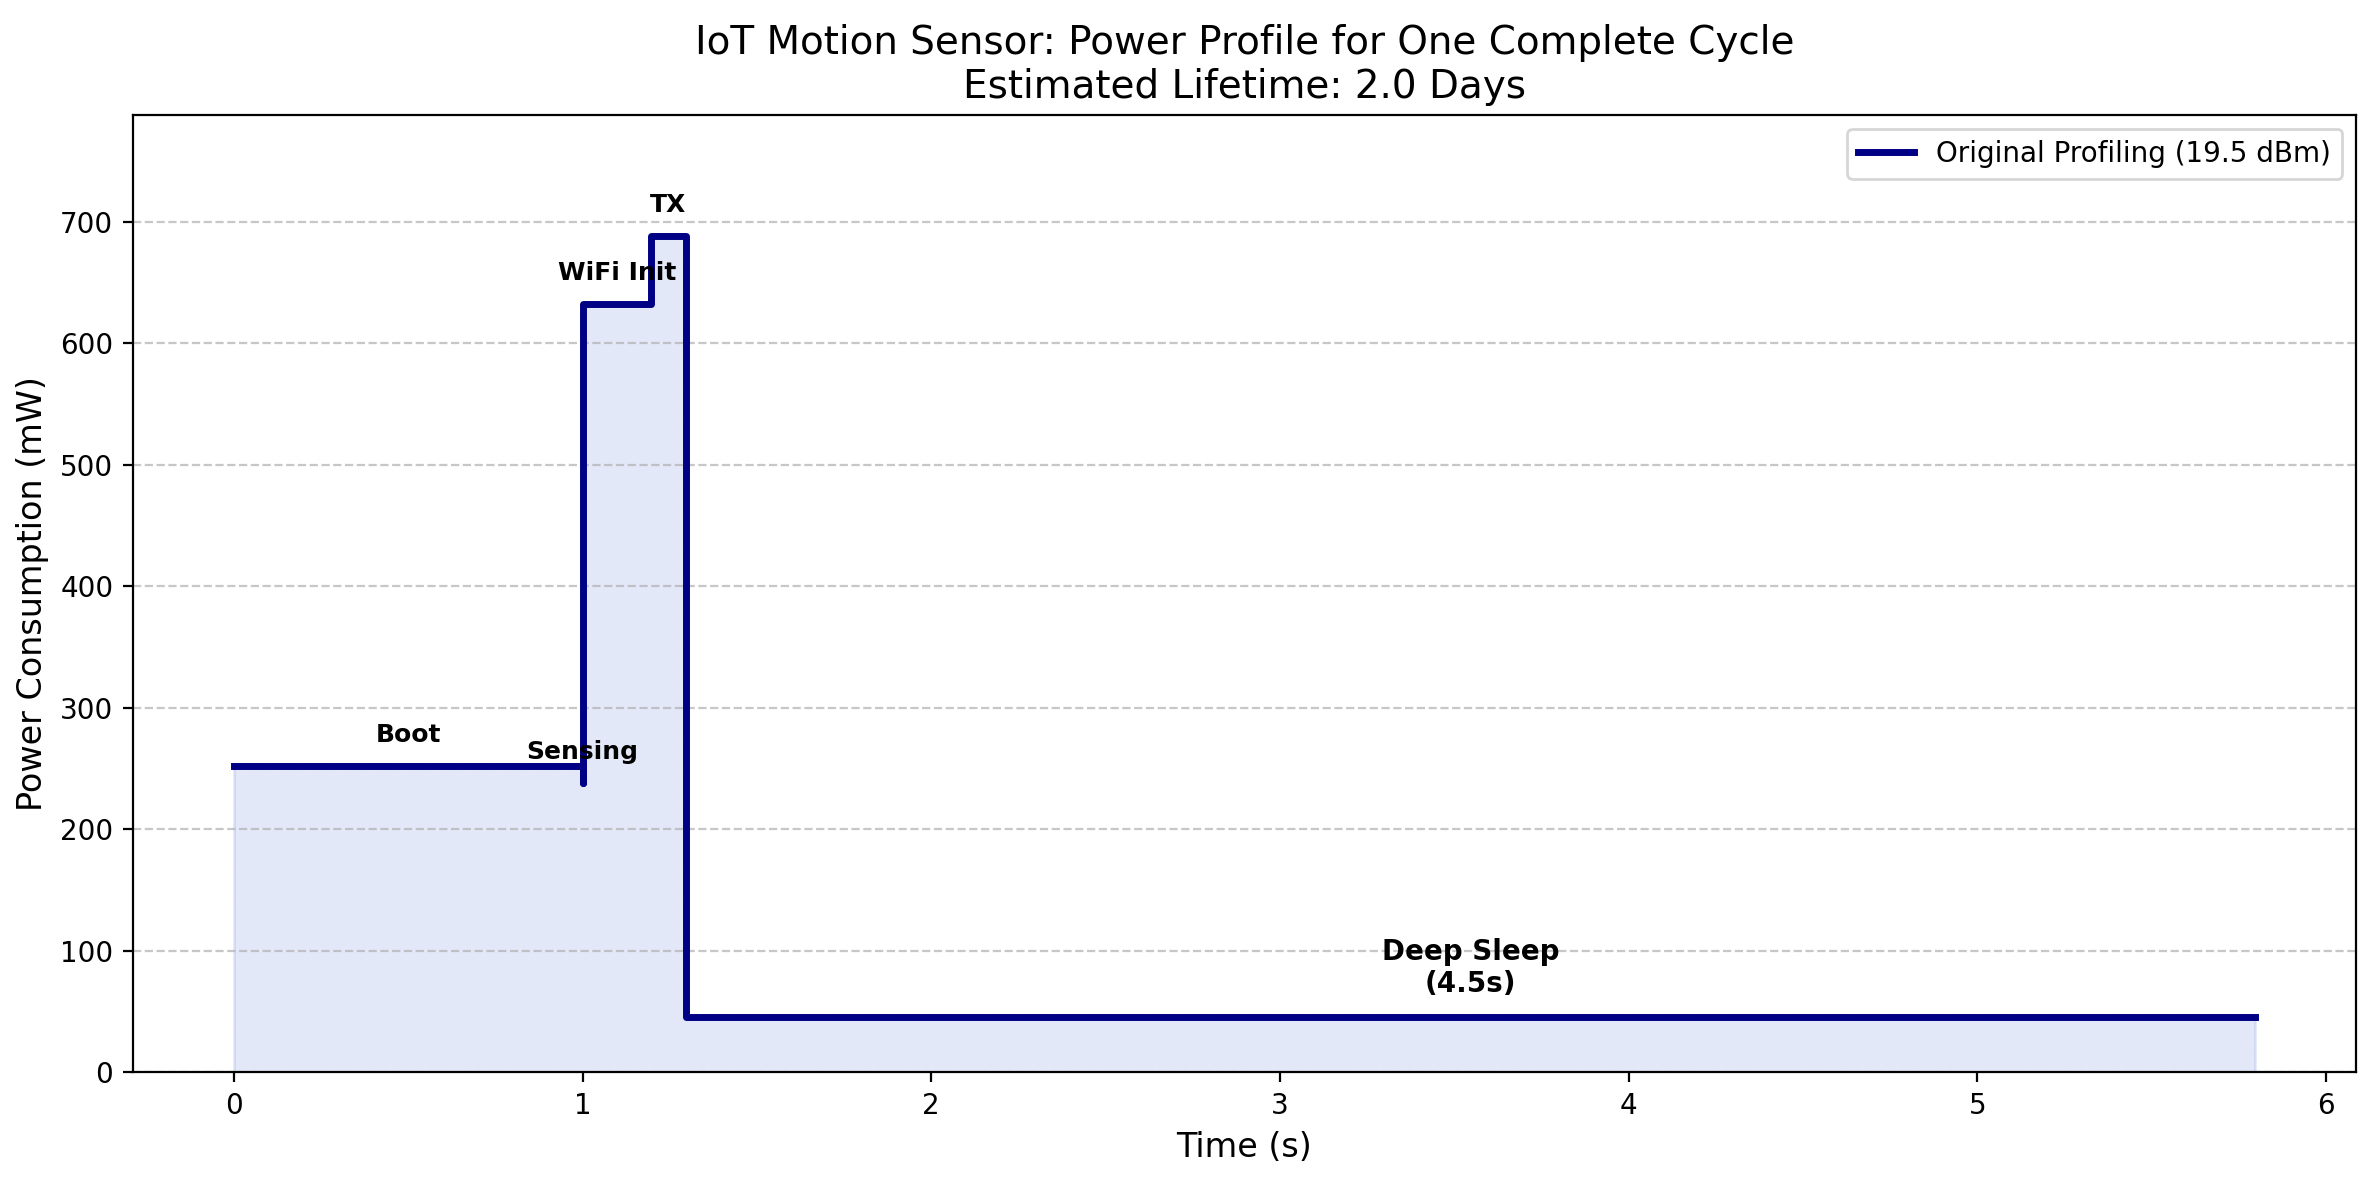
\includegraphics[width=\textwidth]{image/plot1.png}
    \caption{Power consumption over one duty cycle}
\end{figure} 

% ============================================================
\section{Battery Lifetime Estimation}
% ============================================================

The battery energy value $Y$ computed from the team leader's person code (10889590) is  $\mathbf{19590\text{ J}}$. 
The total number of duty cycles supported by the battery is computed as:
$$N = \frac{Y}{E_{\text{cycle}}} = \frac{19590\text{ J}}{0.650\text{ J}} \approx 30115 \text{ cycles}$$
The total operating lifetime is calculated as:
$$T = N \times t_{\text{cycle}} = 30115 \times 5.796\text{ s} \approx 174537\text{ s}$$
Converting this value into days yields an estimated operating lifetime of:
$$T_{\text{days}} = \frac{174537\text{ s}}{86400\text{ s/day}} \approx 2.02 \text{ days}$$

% ============================================================
\section{Improved Version of the Code}
% ============================================================

Three concrete modifications were identified and applied to reduce energy consumption while keeping the node's functionality and communication protocol unchanged. All three are visible in the improved source code and are marked with \texttt{[IMPROVEMENT]}
comments.

\subsection{Reducing the Initial Delay after \texttt{Serial.begin()}}

The original code waits one full second at the beginning of every cycle, immediately after initializing the serial interface:

\begin{lstlisting}[language=C++]
Serial.begin(115200);
delay(1000);   // 1 second wasted at every wake-up
\end{lstlisting}

This delay was introduced to let the serial monitor stabilize before printing
diagnostic messages, and is harmless during development.\\

However, because the ESP32 performs a full reset at every wake-up from Deep Sleep, this line is executed at the beginning of every duty cycle, not only at the first boot. With a cycle period of approximately 5.8 seconds, this single delay accounts for more than 17\% of the total cycle time and consumes 0.252\,J of the 0.651\,J budget per cycle, making it the single largest waste in the entire system.\\

In the improved version the delay is reduced from 1000\,ms to 10\,ms, which is
sufficient to avoid serial glitches while eliminating virtually all of the wasted
active time:

\begin{lstlisting}[language=C++]
Serial.begin(115200);
// [IMPROVEMENT] Reduce initial delay from 1 s to 10 ms
delay(10);
\end{lstlisting}

\begin{table}[H]
\centering
\begin{tabular}{lcc}
\toprule
\textbf{Metric} & \textbf{Before} & \textbf{After} \\
\midrule
Boot energy        & 0.252\,J  & 0.003\,J \\
Energy per cycle   & 0.651\,J  & 0.401\,J \\
Estimated lifetime & 2.02 days & 2.72 days \\
\bottomrule
\end{tabular}
\caption{Impact of reducing \texttt{delay(1000)} to \texttt{delay(10)}: energy per cycle drops by 0.249\,J, the single largest saving among the three improvements.}
\end{table}

\subsection{Lowering the Transmission Power to 2\,dBm}

The default ESP-NOW transmission power on the ESP32 is 19.5\,dBm, which draws
approximately 688\,mW during the transmission phase.\\

Since the challenge specification states that the sink node is always reachable, there is no need to operate at maximum power. The transmission power is reduced to the minimum supported value of 2\,dBm by adding a single API call immediately after \texttt{esp\_now\_init()}, made possible by including \texttt{esp\_wifi.h}:\\

\begin{lstlisting}[language=C++]
esp_now_init();
// [IMPROVEMENT] Reduce TX power from 19.5 dBm to 2 dBm
esp_wifi_set_max_tx_power(8); // 8 x 0.25 dBm = 2 dBm
\end{lstlisting}

At 2\,dBm the transmission phase draws approximately 618\,mW instead of 688\,mW,
reducing the instantaneous power by about 70\,mW during the entire TX window.
The transmission duration does not change, so the energy saving per cycle is directly
proportional to this power difference.

\begin{table}[H]
\centering
\begin{tabular}{lcc}
\toprule
\textbf{Metric} & \textbf{Before} & \textbf{After} \\
\midrule
TX power           & 688\,mW   & 617.880\,mW \\
TX energy          & 0.068\,J  & 0.061\,J \\
Energy per cycle   & 0.651\,J  & 0.644\,J \\
Estimated lifetime & 2.02 days & 2.04 days \\
\bottomrule
\end{tabular}
\caption{Impact of lowering TX power to 2\,dBm: modest but entirely zero-cost saving
that requires a single line of code.}
\end{table}

\subsection{Replacing \texttt{delay(100)} with a Flag-Based Wait}

After calling \texttt{esp\_now\_send()}, the original code waits a fixed 100\,ms to ensure that the \texttt{OnDataSent} callback fires before the node enters Deep Sleep.\\

In practice, ESP-NOW completes the transmission in a few milliseconds, so the
remainder of the delay is wasted with the WiFi radio still active. The improvement introduces a \texttt{volatile} boolean flag \texttt{messageSent},
declared at file scope, which is set to \texttt{true} by the callback as soon as the transmission is confirmed.\\ 

A polling loop then exits immediately once the flag is raised, with a safety timeout of 50\,ms to prevent the node from stalling indefinitely in case of failure:

\begin{lstlisting}[language=C++]
// [IMPROVEMENT] volatile flag instead of a fixed delay
volatile bool messageSent = false;

void OnDataSent(const wifi_tx_info_t *mac_addr,
                esp_now_send_status_t status) {
  Serial.print("[TX] Send Status: ");
  Serial.println(status == ESP_NOW_SEND_SUCCESS ? "Ok" : "Error");
  // [IMPROVEMENT] signal that transmission has ended
  messageSent = true;
}

// After esp_now_send(), instead of delay(100):
unsigned long t_wait = millis();
while (!messageSent && millis() - t_wait < 50) {
  delay(1);
}
\end{lstlisting}

This reduces the TX phase duration from approximately 99\,ms to approximately
1.26\,ms on average, saving around 98\,ms of active time per cycle during which
the WiFi radio would otherwise remain unnecessarily powered on.

\begin{table}[H]
\centering
\begin{tabular}{lcc}
\toprule
\textbf{Metric} & \textbf{Before} & \textbf{After} \\
\midrule
TX duration        & $\sim$99\,ms   & $\sim$1.26\,ms \\
TX energy          & 0.068\,J  & 0.001\,J \\
Energy per cycle   & 0.651\,J  & 0.583\,J \\
Estimated lifetime & 2.02 days & 2.22 days \\
\bottomrule
\end{tabular}
\caption{Impact of the flag-based wait: TX duration drops by $\sim$98\,ms,
saving 0.067\,J per cycle.}
\end{table}

It is worth noting that the callback signature used in this project is
\texttt{const wifi\_tx\_info\_t*}, which corresponds to the ESP32 Arduino framework
version~3.x compiled via PlatformIO. The Wokwi web simulator still uses the older
\texttt{const uint8\_t*} signature from version~2.x, so the same code may not
compile on the web interface without adjusting this parameter type.

\subsection{Increasing the Deep Sleep Duration}

The deep sleep duration $X = 4.5$\,s was imposed by the challenge formula and is not
a free design parameter in this implementation. However, from an application
standpoint, a smart-home motion sensor does not need to report its status multiple
times per second. Human activity in a room changes on a timescale of seconds to
minutes, so a wake-up interval of 30 or 60 seconds would be entirely sufficient
without any meaningful loss of responsiveness.

Since Deep Sleep is the most energy-efficient state by far, increasing its duration
directly reduces the average power consumption proportionally. As an illustrative
example, extending the sleep interval to 60\,s, combined with the three improvements
above, would bring the estimated lifetime from 3.2 to 4.75 days, approaching the
theoretical maximum of approximately 5 days achievable if the node were always in
Deep Sleep.

\begin{table}[H]
\centering
\begin{tabular}{lcc}
\toprule
\textbf{Metric} & \textbf{Sleep 4.5\,s (spec)} & \textbf{Sleep 60\,s (relaxed)} \\
\midrule
Energy per cycle   & 0.333\,J  & 2.874\,J \\
Estimated lifetime & 3.2 days  & 4.75 days \\
\bottomrule
\end{tabular}
\caption{Effect of extending Deep Sleep to 60\,s on top of all other improvements.
The higher per-cycle energy is offset by the much lower wake-up frequency, resulting
in a significantly longer battery lifetime.}
\end{table}

It is worth clarifying why a longer sleep interval leads to a longer battery lifetime even though the energy consumed per cycle increases. What ultimately determines battery lifetime is the average power drawn over time, not the energy per cycle in isolation. The dominant cost in each duty cycle is the WiFi initialization phase, which draws approximately 632\,mW for a fixed 196\,ms regardless of how long the node sleeps afterward. By extending the sleep interval to 60\,s, this fixed overhead is paid 13$\times$ less frequently and is therefore diluted over a much larger time window, reducing the average power significantly. The primary function of the node is also preserved: a 60-second sampling period is entirely adequate for a smart-home motion sensor.

\subsection{Transmitting Only on Status Change}

In the current implementation the node transmits a new message at every wake-up, regardless of whether the sensed conditions have changed since the previous cycle.\\

In a typical smart-home scenario, the state of a room remains constant for extended periods, so most transmissions carry redundant information and consume energy unnecessarily.\\

A more efficient strategy would be to store the last transmitted state in RTC memory, which survives Deep Sleep, and send a new message only when the current reading differs from the previous one. In scenarios where the environment is stable for long periods, this optimization could eliminate the vast majority of transmissions, dramatically extending the battery lifetime without changing the information available to the sink node.

\subsection{Hardware Limitations of the ESP32 Architecture}

It is worth noting that the ESP32, while widely used in IoT prototyping, is not
optimized for ultra-low-power sensing applications. Its Deep Sleep current is
acceptable (10--150\,$\mu$A), but the 200\,ms wake-up and radio initialization
overhead is inherent to the architecture and cannot be reduced through software alone.
For a production deployment, migrating to a more power-efficient platform would
represent the most impactful long-term improvement.

% ============================================================
\section{Comparison Between Original and Improved Version}
% ============================================================
 
The three modifications described in the previous section (reducing the boot delay from 1000\,ms to 10\,ms, replacing the fixed \texttt{delay(100)} with a flag-based wait, and lowering the TX power to 2\,dBm ) are all compatible with the challenge constraints and are applied simultaneously in the improved code. \\

Their combined effect on the duty cycle is summarized in Table~\ref{tab:comparison}.
 
\begin{table}[H]
\centering
\begin{tabular}{lrrrr}
\toprule
\textbf{Phase} & \textbf{Power} & \textbf{Time (orig.)} & \textbf{Time (impr.)} & \textbf{Energy (impr.)} \\
\midrule
Boot delay          & 252\,mW & 1000\,ms  & 10\,ms    & 0.003\,J \\
Sensor acquisition  & 238\,mW &  0.43\,ms &  0.43\,ms & 0.000\,J \\
WiFi + ESP-NOW init & 632\,mW &  196\,ms  &  196\,ms  & 0.124\,J \\
Transmission        & 618\,mW &  99.3\,ms &  1.26\,ms & 0.001\,J \\
Deep Sleep          &  46\,mW & 4500\,ms  & 4500\,ms  & 0.206\,J \\
\midrule
Total active time   &  ---    & $\approx$1296\,ms & $\approx$208\,ms & --- \\
Active fraction     &  ---    & $\approx$22\%     & $\approx$4.4\%   & --- \\
\midrule
Energy per cycle    &  ---    & 0.651\,J  & 0.333\,J  & ---      \\
Estimated lifetime  &  ---    & 2.02 days & 3.20 days & ---      \\
\bottomrule
\end{tabular}
\caption{Full comparison between the original and improved implementation.
The power values are those measured from the CSV traces and are shared between the
two versions except for TX, where 618\,mW reflects the reduced 2\,dBm setting.
Deep Sleep power is identical in both versions.}
\label{tab:comparison}
\end{table}
 
The most significant result is the reduction of the active fraction from approximately 22\% down to approximately 4.4\% of the total cycle.\\

Together, the three changes bring the energy per cycle from
0.651\,J to 0.333\,J, increasing the estimated battery lifetime from 2.02 to
3.20 days without any change to the node's sensing and communication behavior: the
same two sensors are read, the same message format is used, and the same ESP-NOW
broadcast protocol delivers the data to the sink node.
 
\begin{figure}[H]
    \centering
    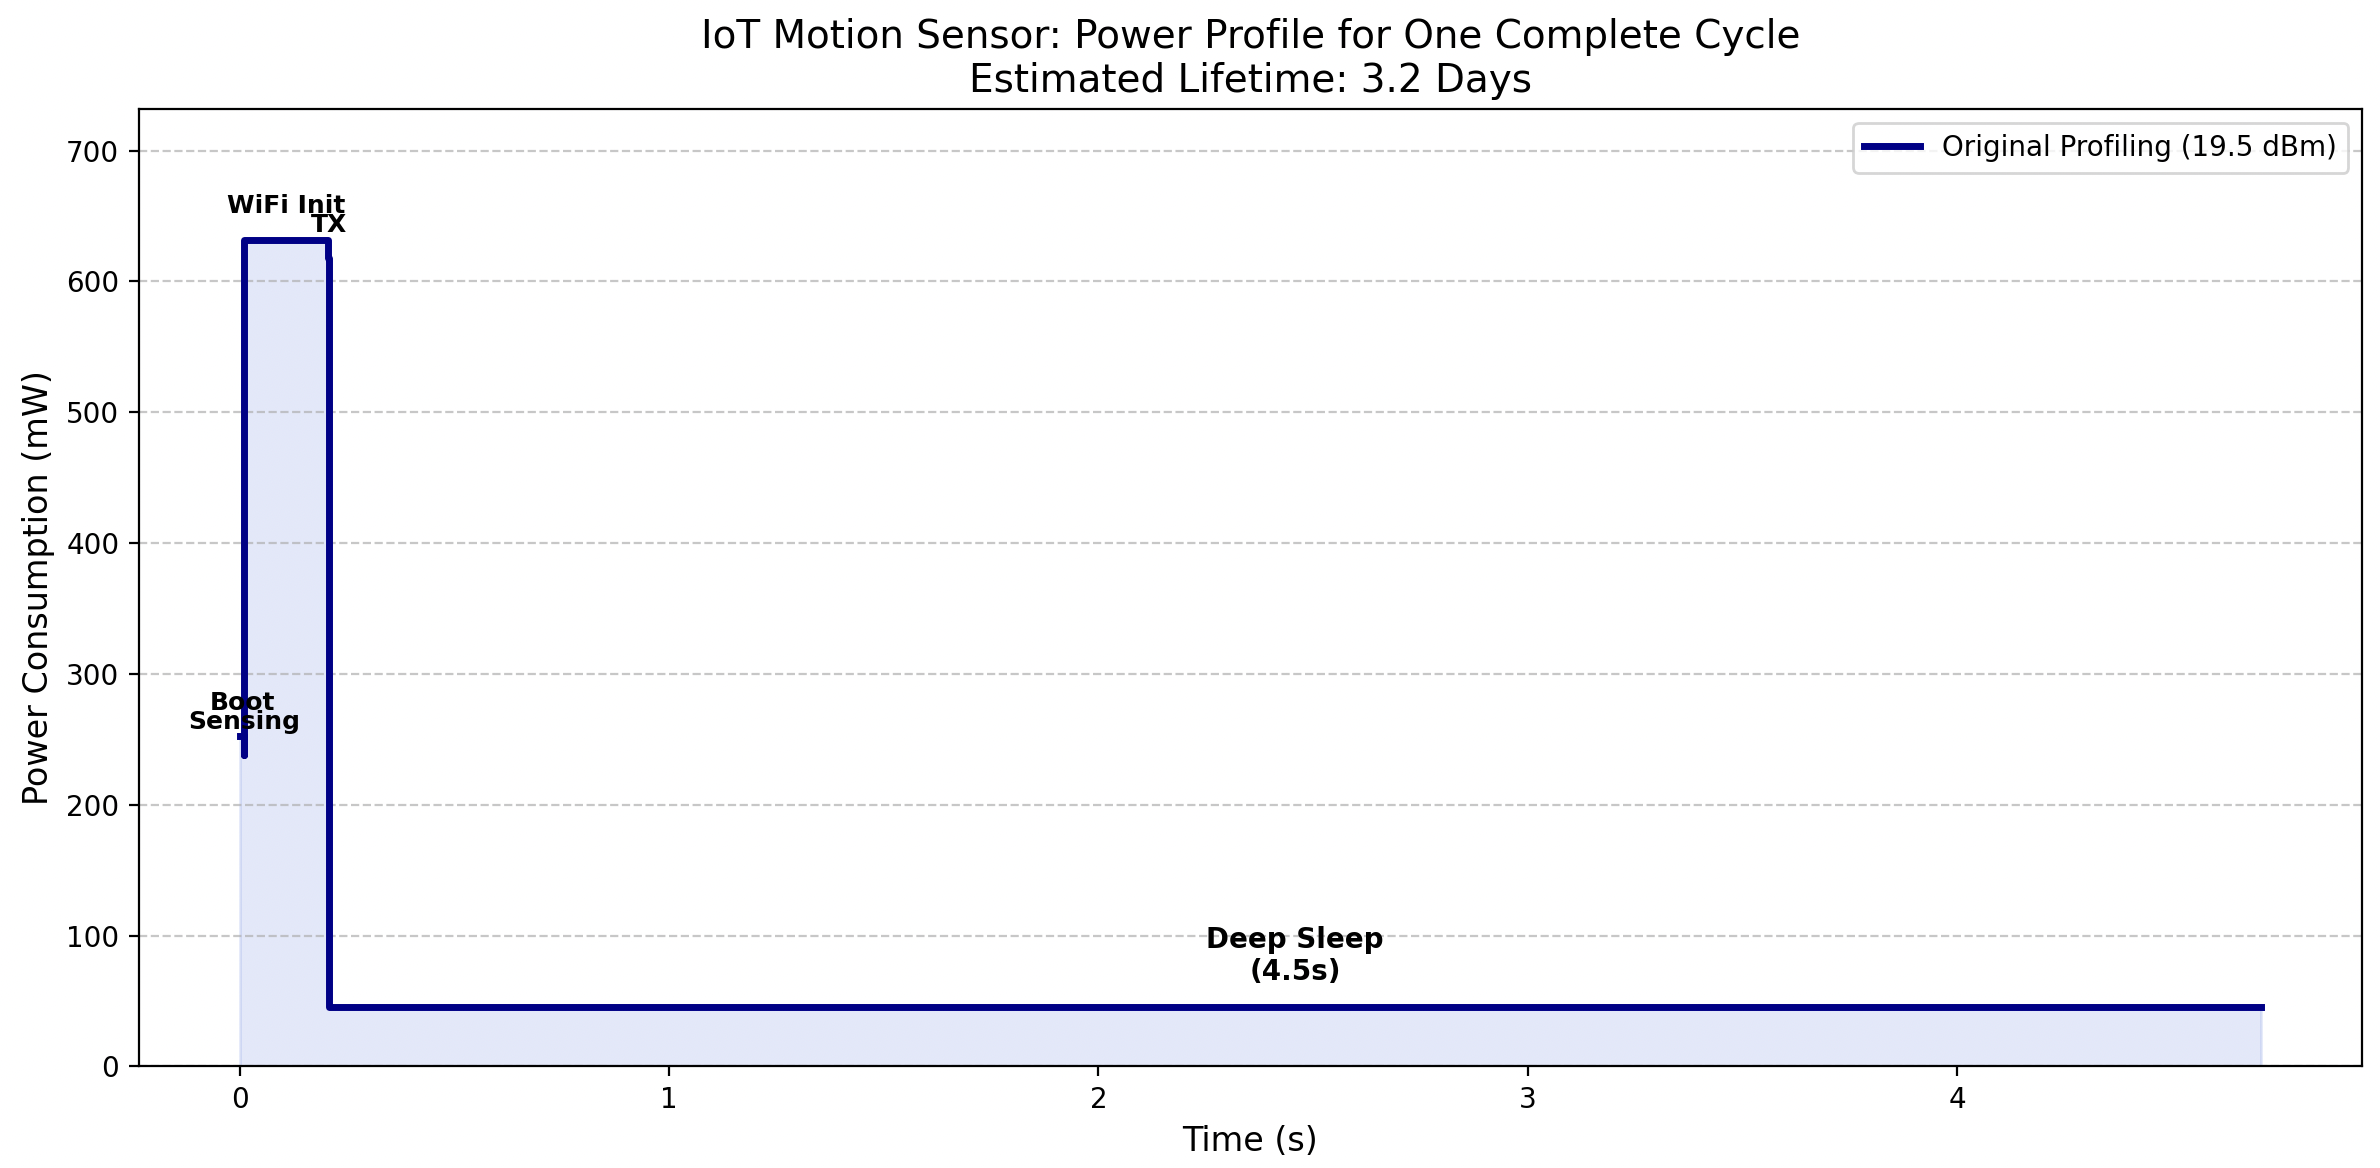
\includegraphics[width=\textwidth]{image/plot2.png}
    \caption{Power consumption of the improved system over one duty cycle}
\end{figure}
 
The power-vs-time graph makes the improvement immediately visible. In the original
version the cycle opens with a 1-second plateau at the idle power level due to the
boot delay, followed by the WiFi initialization peak and a 99\,ms TX window. In the
improved version the boot delay shrinks to 10\,ms and the TX window drops to roughly
1.26\,ms, so the active portion of the graph is dramatically shorter before the node
drops back into Deep Sleep.
 
For completeness, Table~\ref{tab:full_summary} extends the comparison to include the
scenario in which the Deep Sleep interval is also relaxed from 4.5\,s to 60\,s.
Although this configuration goes beyond the challenge constraints, it illustrates the
theoretical upper bound achievable through software-only optimizations on the current
hardware platform. The active fraction in this case drops below 0.35\%, and the
estimated battery lifetime reaches 4.75 days, approaching the theoretical ceiling of approximately 5 days that would be achieved if the node were always in Deep Sleep.
 
\begin{table}[H]
\centering
\begin{tabular}{lrrr}
\toprule
\textbf{Metric} & \textbf{Original} & \textbf{Improved} & \textbf{+ Sleep 60\,s} \\
\midrule
Boot delay             & 1000\,ms   & 10\,ms     & 10\,ms     \\
TX duration            & 99.3\,ms   & 1.26\,ms   & 1.26\,ms   \\
TX power               & 688\,mW    & 618\,mW    & 618\,mW    \\
Deep Sleep             & 4500\,ms   & 4500\,ms   & 60\,000\,ms \\
\midrule
Total active time      & $\approx$1296\,ms & $\approx$208\,ms & $\approx$208\,ms \\
Active fraction        & $\approx$22\%     & $\approx$4.4\%   & $\approx$0.34\%  \\
\midrule
Energy per cycle       & 0.651\,J   & 0.333\,J   & 2.874\,J   \\
Estimated lifetime     & 2.02 days  & 3.20 days  & 4.75 days  \\
\bottomrule
\end{tabular}
\caption{Full three-way comparison: original implementation, improved version
(three software fixes within challenge constraints), and improved version with
Deep Sleep extended to 60\,s (relaxed constraint). The per-cycle energy increases
in the third scenario because the sleep interval is 13$\times$ longer, but the
average power and therefore the battery lifetime both improve significantly.}
\label{tab:full_summary}
\end{table}
 
% ============================================================
\section{Conclusion}
% ============================================================

This work presented the design, simulation, and energy analysis of a duty-cycled
IoT motion sensor node based on the ESP32 platform. The implemented node satisfies
all challenge requirements: it correctly reads motion and ambient light data through
a PIR sensor and a photoresistor, formats the output string according to the
specified syntax, and transmits it to the sink node via the ESP-NOW broadcast
protocol. After each transmission, the board enters Deep Sleep for the interval
$X = 4.5$\,s derived from the team leader's person code, and wakes up again to
repeat the cycle.\\

The energy analysis confirmed that wireless communication is by far the most
demanding component of the duty cycle. The WiFi and ESP-NOW initialization phase
alone draws over 630\,mW for nearly 200\,ms at every wake-up, and this cost is
essentially fixed: it cannot be avoided as long as ESP-NOW is used, and it cannot
be reduced through software tuning alone. This highlights a fundamental constraint
of the ESP32 architecture for battery-powered applications.\\

Deep Sleep, on the other hand, is the key enabler of long battery lifetime. At
roughly 46\,mW, the power drawn during sleep is more than an order of magnitude
lower than during active operation. Since the node spends the majority of its time
in this state, even modest reductions in active time translate into meaningful
improvements in overall efficiency. The three software optimizations applied in
this work, eliminating the wasteful boot delay, replacing the fixed
\texttt{delay(100)} with a flag-based wait, and lowering the transmission power to
2\,dBm, together reduce the active fraction from approximately 22\% to 4.4\%
and cut the energy per cycle from 0.651\,J to 0.333\,J, extending the estimated
battery lifetime from 2.02 to 3.20 days.\\

These results demonstrate that even simple, zero-cost software changes can have a
significant impact on the energy budget of a constrained IoT device, provided that
the sources of waste are correctly identified through measurement rather than
guesswork.
 
\end{document}
 